\documentclass[11pt]{article}

% ---- Packages ----------------------------------------------------------------
\usepackage[T1]{fontenc}
\usepackage{lmodern}
\usepackage[margin=1in]{geometry}
\usepackage{amsmath,amssymb,amsthm}
\usepackage{booktabs}
\usepackage{graphicx}
\usepackage{xcolor}
\usepackage[authoryear,round]{natbib}
\usepackage[colorlinks=true,allcolors=blue!60!black]{hyperref}
\usepackage[capitalise,noabbrev]{cleveref}

\graphicspath{{figures/}}

\hypersetup{
  pdftitle={Fewer Giants, More Firms? Artificial Intelligence, Entry Costs, and the Firm Size Distribution},
  pdfkeywords={artificial intelligence, cloud computing, firm entry, firm size distribution, business dynamism}
}

% ---- Theorem-like environments -----------------------------------------------
\theoremstyle{plain}
\newtheorem{proposition}{Proposition}
\theoremstyle{definition}
\newtheorem{assumption}{Assumption}
\newtheorem{definition}{Definition}
\newtheorem{prediction}{Prediction}
\crefname{assumption}{Assumption}{Assumptions}
\crefname{prediction}{Prediction}{Predictions}

% ---- Macros ------------------------------------------------------------------
% Visible marker for text the author still has to write; remove before submission.
\newcommand{\placeholder}[1]{\textcolor{gray}{[\textit{#1}]}}
% Size classes: L = large incumbents, B = the 5--4,999 band, S = fewer than 5 employees.
\newcommand{\Lc}{\mathcal{L}}
\newcommand{\Bc}{\mathcal{B}}
\newcommand{\Sc}{\mathcal{S}}

% ---- Front matter ------------------------------------------------------------
\title{Fewer Giants, More Firms?\\Artificial Intelligence, Entry Costs, and the Firm Size Distribution\thanks{\placeholder{Acknowledgments, funding, data access, and AI-use disclosure statement.}}}
\author{Gerard Spivey\\\href{mailto:gs@gspivey.com}{gs@gspivey.com}}
\date{\placeholder{Preliminary draft} --- \today}

\begin{document}

\maketitle

\begin{abstract}
\noindent
Artificial intelligence (AI) raises the productivity of incumbent firms, and a prominent concern is that large firms will use these gains to reduce headcount.
Less attention has been paid to a second margin of adjustment: whether AI also lowers the cost of starting and scaling a new firm.
We argue that the closest historical precedent is cloud computing, which converted the fixed cost of computing infrastructure into a variable cost and thereby reduced the capital required to launch a firm.
This paper asks whether AI-induced firm formation can offset the employment that large incumbents shed.
We develop a model of firm dynamics with endogenous entry and exit in which the AI shock has two components: a labor-saving change in the technology of incumbents and a reduction in the fixed costs of entry and operation.
We discipline the entry-cost component using the cloud-computing era (2006--2020), calibrate the model to US business-dynamism moments, and use Monte Carlo simulation to characterize the conditions under which job creation at small and mid-sized firms and entrants offsets displacement at large incumbents.
The cloud era is a cautionary precedent: lower computing costs coincided with rising employment concentration and a falling startup rate, a pattern the model reproduces only when a labor-complementary technology is combined with entry headwinds.
Across 2,000 Monte Carlo draws, the probability that AI raises net employment is 81.7\%, but this headline is conditional: the labor-AI substitution elasticity explains 71\% of the variance in employment outcomes, while entry-cost reduction explains only 3\%.
Below a displacement threshold ($\sigma_{\text{ai}} < 2.78$), offset is nearly universal (99.8\%); above it, offset depends on whether AI-native entrants are substantially more productive.
We derive empirical signatures that distinguish offsetting entry from pure displacement and map them to administrative business data.
Early survey evidence suggests AI is currently labor-complementary at adopting firms, but AI-native firms are markedly employment-light, and business applications with planned wages are falling even as total applications reach record highs.
\end{abstract}

\medskip
\noindent\textbf{JEL codes:} D22, E24, J23, L11, L26, O33.\\
\noindent\textbf{Keywords:} artificial intelligence, cloud computing, firm entry, firm size distribution, business dynamism, labor displacement.

\newpage

% ---- Body --------------------------------------------------------------------
\section{Introduction}\label{sec:intro}

% ---- P1. The problem -------------------------------------------------------
Firms are adopting artificial intelligence (AI) rapidly, and early experimental and field evidence documents sizable productivity gains in specific tasks \citep{noy2023experimental,brynjolfsson2025generative}.
If these gains are labor-saving at the firm level, the first-order prediction is that incumbents will produce the same output with fewer workers \citep{acemoglu2019automation}.
The concern is sharpest for large firms, which have the data, capital, and organizational capacity to adopt early: in the European Union in 2025, 55\% of enterprises with 250 or more employees used AI, against 17\% of those with 10 to 49 employees \citep{eurostat2026isoc}.
This paper is about the second-order response.
A technology that makes existing firms more productive may also make new firms cheaper to create.
We ask whether, when AI reduces headcount at large incumbents, it also lowers the barriers to firm formation enough that employment in new small and mid-sized firms offsets the displacement.

% ---- P2. Why it matters ----------------------------------------------------
The answer matters for how economists and policymakers read the labor-market consequences of AI.
Most existing assessments measure the exposure of occupations and tasks \citep{eloundou2024gpts,acemoglu2025simple}, implicitly holding the set of firms fixed.
Yet net job creation in the United States is driven disproportionately by young firms rather than by small firms as such \citep{haltiwanger2013who}, and the long decline in business dynamism has been linked to slower reallocation and weaker productivity growth \citep{decker2014role,decker2020changing}.
If AI moves the entry margin, changes in the number and size of firms could rival the within-firm displacement that task-based accounts emphasize.
The question is equally pressing in Europe, where firm size distributions, entry costs, and labor-market institutions differ from those in the United States \citep{bartelsman2013cross}, and where a new regulatory framework for AI is being phased in \citep{euaiact2024}.

% ---- P3. Why it is hard ----------------------------------------------------
Answering the question is hard for three reasons.
First, AI is still diffusing, so the post-shock firm size distribution is not yet observed and any direct test is necessarily partial.
% [claim] speed asymmetry is plausible but should be supported (e.g. entrant scale-up horizons in BDS).
Second, the two channels operate at different speeds: incumbents can cut headcount within a budget cycle, whereas the entry, survival, and scale-up of new firms unfold over years, so short-run data will tend to overstate net displacement.
Third, the natural historical comparison is not clean: the cloud era coincided with a secular decline in the aggregate US startup rate \citep{decker2016declining,akcigit2021ten}, so any entry effect of cloud computing must be identified within exposed sectors and against a falling baseline rather than read off aggregate series.
A naive before-and-after comparison of aggregate employment therefore conflates the two channels and confounds both with unrelated trends.

% ---- P4. The gap and how this paper differs ---------------------------------
Prior work has studied each channel largely in isolation.
A large literature on automation studies displacement and reinstatement of labor within a given set of firms or industries \citep{autor2003skill,autor2015why,acemoglu2018race}, and work on superstar firms documents rising concentration alongside a falling labor share \citep{autor2020fall}.
Research on information technology shows that its effects depend on how firms are organized \citep{bloom2012americans,bloom2014distinct}, and recent evidence links AI investment to firm growth and product innovation \citep{babina2024artificial}.
Separately, research on cloud computing shows that cheaper experimentation changed how startups are financed \citep{ewens2018cost} and affected the survival and performance of young establishments \citep{jin2017economies}.
Canonical models of firm dynamics connect entry costs to the firm size distribution \citep{hopenhayn1992entry,luttmer2007selection}.
% [claim] "to our knowledge" requires a completed literature search before submission.
To our knowledge, these models have not been used to ask whether a shock that combines labor-saving technical change with lower entry costs raises or lowers aggregate employment.
We bring these strands together and use cloud computing as a disciplined analogue for the entry-cost component of the AI shock.

% ---- P5. What we do, what we find, and the limits --------------------------
We proceed in four steps.
We first set out a model of firm dynamics with endogenous entry and exit (\cref{sec:theory}).
We then use the cloud era of 2006--2020 to ask which parameter configurations reproduce what happened: lower computing costs coincided with rising employment concentration and a falling startup rate, a pattern the model matches only when a labor-complementary technology is combined with entry headwinds (\cref{sec:cloud}).
Next, we formalize the AI shock as a combination of displacement at incumbents and lower fixed costs of entry and operation (\cref{sec:ai-model}), and we calibrate the model and simulate it by Monte Carlo (\cref{sec:simulation}).
We find that the probability that AI raises net employment is 81.7\%, but the result is conditional: whether AI is labor-complementary ($\sigma_{\text{ai}} < 2.78$) or labor-displacing explains 71\% of the variance, while entry-cost reduction---the mechanism most analogous to cloud computing---explains only 3\%.
Below the displacement threshold, offset is nearly universal; above it, offset depends on whether AI-native entrants are substantially more productive than they would have been absent AI.
Finally, we derive empirical signatures that can be tested as AI diffuses (\cref{sec:signatures}).
Our analysis has clear limits: the analogy to cloud computing is imperfect, and because AI can substitute for labor at entrants as well as at incumbents, more firms need not mean more jobs.
In the discussion (\cref{sec:discussion}) we distinguish AI infrastructure providers (labs, hyperscalers) from AI application companies and document that the leading application firms are far more employment-light than cloud-era software firms: Cursor generates more than twenty times the revenue per employee of cloud-era SaaS comparators.

\paragraph{Contributions.}
This paper makes four contributions.
\begin{itemize}
  \item \textbf{A two-channel model of the AI shock.}
  We embed labor-saving technical change at incumbents and lower fixed costs of entry and operation in a single model of firm dynamics, so that displacement and firm formation are determined jointly rather than studied in isolation.
  \item \textbf{Cloud computing as an empirical analogue.}
  We use the 2006--2020 cloud era in the United States and Europe to discipline the entry-cost channel, accounting for the concurrent decline in business dynamism.
  \item \textbf{Quantitative conditions for offset.}
  We characterize, by calibration and Monte Carlo simulation, the conditions under which employment among firms with 5 to 4,999 employees offsets displacement at large incumbents.
  \item \textbf{Testable empirical signatures.}
  We derive predictions that distinguish offsetting entry from pure displacement and map each one to existing US and European administrative data.
\end{itemize}

The remainder of the paper is organized as follows.
\Cref{sec:theory} presents the framework, \cref{sec:cloud} studies the cloud era, \cref{sec:ai-model} formalizes the AI shock, \cref{sec:simulation} reports the calibration and simulations, \cref{sec:signatures} states the empirical signatures, \cref{sec:discussion} discusses limitations and policy, and \cref{sec:conclusion} concludes.

\section{Theoretical Framework}\label{sec:theory}

% Role: baseline environment without AI; the shock is added in sec:ai-model.
We embed a span-of-control technology \citep{lucas1978size} in an entry-and-exit model \citep{hopenhayn1992entry}, a structure chosen because it links entry and operating costs directly to the firm size distribution.
The model is a workhorse in the business dynamism literature \citep{decker2014role,haltiwanger2013who}, and its extension with random growth yields a Pareto tail that matches the observed right skew of the firm size distribution \citep{luttmer2007selection,axtell2001zipf}.

\subsection{Environment}\label{sec:theory-env}

Time is discrete.
A continuum of firms produces a homogeneous good using labor, with idiosyncratic productivity $z$ that follows an AR(1) process in logs,
\begin{equation}\label{eq:productivity-process}
  \ln z' = \rho \ln z + (1-\rho)\mu + \varepsilon, \qquad \varepsilon \sim \mathcal{N}(0, \sigma_z^2),
\end{equation}
with persistence $\rho$ and long-run mean $\mu$.
A firm with productivity $z$ that employs $n$ workers produces
\begin{equation}\label{eq:production}
  y = z\, n^{\alpha}, \qquad 0 < \alpha < 1,
\end{equation}
where $\alpha$ is the span-of-control parameter (decreasing returns to labor), and pays the wage $w$ and a fixed operating cost $c_f$ each period.

\subsection{Incumbents}\label{sec:theory-incumbents}

Static profit maximization gives labor demand
\begin{equation}\label{eq:labor-demand}
  n(z) = \left( \frac{\alpha z}{w} \right)^{\frac{1}{1-\alpha}},
\end{equation}
and the value of an incumbent satisfies
\begin{equation}\label{eq:value}
  V(z) = \pi(z) - c_f + \beta \int \max\bigl\{ 0,\, V(z') \bigr\}\, dF(z' \mid z),
\end{equation}
where $\pi(z)$ is static profit before the fixed cost and $\beta$ is the discount factor.
Firms exit when $V(z) < 0$, which defines an exit threshold $z^{*}$.

\subsection{Entry}\label{sec:theory-entry}

A potential entrant pays a sunk entry cost $c_e$ and then draws initial productivity from a distribution $G(z)$.
With positive entry in equilibrium, free entry requires
\begin{equation}\label{eq:free-entry}
  \int V(z)\, dG(z) = c_e .
\end{equation}

\subsection{Stationary equilibrium and employment accounting}\label{sec:theory-equilibrium}

A stationary equilibrium is a wage $w$, a mass of entrants $M_e$, an exit threshold $z^{*}$, and an invariant distribution of firms $\mu$ such that \cref{eq:labor-demand,eq:value,eq:free-entry} hold and the labor market clears.
In the baseline we take labor supply to be perfectly elastic at the wage $w$, so that displacement shows up as lower employment rather than lower wages; \cref{sec:disc-limitations} discusses how a finite labor-supply elasticity would change the results.

We partition firms by employment into three size classes: large incumbents $\Lc$ (5,000 employees or more), the band of small and mid-sized firms $\Bc$ (5 to 4,999 employees), and very small firms $\Sc$ (fewer than 5).
Aggregate employment is then
\begin{equation}\label{eq:employment}
  N = N^{\Lc} + N^{\Bc} + N^{\Sc}, \qquad N^{k} = \int_{z:\, n(z) \in k} n(z)\, d\mu(z), \quad k \in \{\Lc, \Bc, \Sc\}.
\end{equation}
% [rigor] The 5,000 cutoff matches BDS firm-size classes; European data are typically top-coded at 250+. See sec:cloud-data.
\Cref{eq:employment} is an accounting identity; the model's content is in how a shock moves firms across the size classes and changes the mass of firms in each one.

\subsection{The displacement threshold}\label{sec:theory-threshold}

The model has a key threshold that governs whether technological change raises or lowers employment.
We show in \cref{sec:ai-ces} that when AI is modeled as a substitute for labor within a CES production bundle with elasticity of substitution $\sigma_{\text{ai}}$, AI adoption \emph{increases} a firm's headcount if and only if
\begin{equation}\label{eq:threshold}
  \sigma_{\text{ai}} < \frac{1}{1-\alpha} \equiv \theta.
\end{equation}
With $\alpha = 0.64$ (a standard calibration from \citealp{hopenhayn1993job}), the threshold is $\theta \approx 2.78$.
Below this threshold, the scale effect dominates: cheaper effective input lets the firm produce more, and the extra output requires more labor.
Above the threshold, the substitution effect dominates: the firm replaces workers with AI services faster than it grows.

This parameter---the labor-AI substitution elasticity---will prove to be the central uncertain quantity.
% [claim] Verify that Graetz and Michaels (2018) report elasticities in this range; their headline results are productivity and employment effects, not substitution elasticities.
Existing estimates of automation elasticities range from 0.3 to 1.7 for robots \citep{graetz2018robots}, though these pertain to physical automation rather than AI.
More recent surveys suggest AI adoption has not yet triggered employment reductions at adopting firms: the Census Bureau's Business Trends and Outlook Survey (October 2026) reports that only 2\% of AI-adopting establishments reduced employment due to AI, while 4.7\% increased headcount \citep{btos2026oct}.
We therefore treat $\sigma_{\text{ai}}$ as uncertain and explore its effects through Monte Carlo simulation (\cref{sec:simulation}).

\section{The Cloud Computing Parallel, 2006--2020}\label{sec:cloud}

% Role: empirical analogue that disciplines the entry-cost channel (kappa_e, kappa_f in sec:ai-model).

\subsection{Why cloud computing is the right analogue}\label{sec:cloud-why}

Before commercial cloud services, a new technology firm had to buy and operate its own servers before it could test whether its product had demand.
The public launch of Amazon Web Services' storage and compute services in 2006 allowed firms to rent computing capacity by the unit instead, converting a fixed, sunk investment into a variable cost.
\citet{ewens2018cost} exploit this change and show that lower costs of experimentation altered how venture investors financed early-stage firms in the affected sectors.
In the model of \cref{sec:theory}, this shock maps naturally into a reduction of the entry cost $c_e$ and the fixed operating cost $c_f$, with no direct change in the labor requirement of incumbents.
This is the sense in which cloud computing isolates one of the two channels of the AI shock.
\placeholder{Add evidence on cloud adoption by firm size and age, for example \citet{jin2017economies}, and on the timing of diffusion in Europe relative to the United States.}

\subsection{Data}\label{sec:cloud-data}

We draw on multiple sources to characterize the cloud era.
For the United States: the Census Bureau's Business Dynamics Statistics (BDS) provides firm and establishment entry, exit, and employment by firm size and age annually from 1978--2021 \citep{bds2021}; the Business Formation Statistics (BFS) track business applications and planned-wage intentions from 2004 \citep{bfs2026}.
For Europe: Eurostat Structural Business Statistics and business demography statistics cover EU member states, and the OECD DynEmp database provides harmonized firm-level aggregates.

Size-class definitions differ across sources.
The upper bound of the band $\Bc$ aligns with the firm-size classes in the US data (5,000 employees), whereas European aggregate statistics typically group all firms with 250 or more employees, so the European analysis uses a narrower band where necessary.

\subsection{Empirical findings: cloud produced concentration, not offset}\label{sec:cloud-findings}

The 2006--2020 cloud era provides a cautionary baseline.
Contrary to the hypothesis that lower fixed costs would proliferate small firms, US employment became more concentrated \citep{bds2021}:

\begin{itemize}
  \item \textbf{Small-firm employment share fell}: from 50.9\% (2006) to 47.0\% (2019) for firms with fewer than 500 employees, and about 90\% of the net rise in employment over the period occurred at firms with 500 or more employees.
  \item \textbf{The startup rate declined}: the employer startup rate fell from 10.3\% (2006) to 8.5\% (2019), and the employment share of young firms (five years or younger) fell from 13.4\% to 10.6\%, continuing a secular decline that predates cloud computing \citep{decker2016declining}.
  \item \textbf{The largest firms gained share}: firms with 10,000 or more employees raised their share of employment from 26.3\% to 29.2\%, consistent with the rise of superstar firms documented by \citet{autor2020fall}.
  \item \textbf{Formation shifted to the nonemployer margin}: business applications rose 34\% between 2006 and 2019, while applications with planned wages fell 48\% \citep{bfs2026}.
\end{itemize}

The most cloud-exposed sector is a partial exception.
The startup rate in Information (NAICS 51) recovered from 8.5\% in 2010 to 11.3\% in 2019, above its 2006 level of 10.6\%, whereas professional services, retail, and manufacturing remained below their 2006 levels \citep{bds2021}.
Cloud computing also enabled notable successes (Airbnb, Stripe, Dropbox), but these firms ``graduated'' into the large-firm category rather than remaining in the small-firm band.

\subsection{Why did cloud fail to offset?}\label{sec:cloud-mechanism}

Our primary use of the cloud era is as a calibration target rather than a causal identification exercise.
We ask what parameter configuration of the model replicates the cloud-era pattern of lower computing costs combined with rising concentration and falling dynamism.
No single entry-side parameter does so: varying the entry cost, the fixed cost, entrant quality, or the founder pool on its own leaves the small-firm share rising.
Matching all three moments requires two ingredients together:

\begin{enumerate}
  \item \textbf{Labor-complementary technology} ($\sigma < \theta \approx 2.78$): adopting firms expand rather than shed labor, so employment shifts toward large adopters. This ingredient alone produces concentration but \emph{raises} the startup rate.
  \item \textbf{Entry headwinds}: a higher net employer entry cost, a smaller pool of potential entrants, and no productivity gain for cloud-native entrants, consistent with the regulatory, demographic, and labor-market forces behind declining dynamism \citep{akcigit2021ten}.
\end{enumerate}

\Cref{tab:cloud-results} reports the best-fitting configuration, which sets $\sigma = 2.0$, raises the employer entry cost by 20\%, and shrinks the founder pool by 20\%.
The two ingredients separate cleanly: the technology parameter drives the size distribution, while the entry-side headwinds drive the decline in dynamism.
Because the model's pre-shock levels are not calibrated to these moments, we compare changes rather than levels.

\begin{table}[t]
  \centering
  \caption{Best-fitting cloud-era configuration: model versus data, 2006--2019}
  \label{tab:cloud-results}
  \begin{tabular}{lcc}
    \toprule
    \multicolumn{3}{l}{\textit{Parameters}} \\
    $\sigma$ (substitution) & \multicolumn{2}{c}{$2.0$ (labor-complementary)} \\
    Employer entry cost & \multicolumn{2}{c}{$+20\%$ (headwinds offset savings)} \\
    Entrant productivity shift & \multicolumn{2}{c}{$0$} \\
    Founder pool & \multicolumn{2}{c}{$-20\%$ (declining dynamism)} \\
    \midrule
    Moment (change) & Model & Data \\
    \midrule
    Employment share of firms $<500$ (pp) & $-2.3$ & $-3.9$ \\
    Startup rate (pp) & $-1.6$ & $-1.8$ \\
    Young-firm employment share (pp) & $-3.1$ & $-2.8$ \\
    \bottomrule
  \end{tabular}
  \smallskip
  \footnotesize\textit{Notes: Model values average years 11--15 after the shock (centered on 2019) across 24 seeds, relative to a no-shock counterfactual. Data from \citet{bds2021}.}
\end{table}

The implication for AI is twofold.
First, even labor-complementary AI ($\sigma_{\text{ai}} < 2.78$) could produce concentration if entry headwinds persist.
Second, the offset found in \cref{sec:simulation} rests on an intact entry pipeline: imposing cloud-era founder headwinds on the baseline AI shock ($\sigma_{\text{ai}} = 3.5$, a 20\% cut in entry costs) turns a long-run net employment gain of about $+4\%$ into a loss of $-8.7\%$ after 13 years and $-15.4\%$ in the long run.

\subsection{Empirical strategy}\label{sec:cloud-strategy}

The calibration exercise disciplines the entry-cost channel while remaining agnostic about identification.
For readers interested in the causal effect of cloud computing on entry, the canonical event-study design compares industries by their ex ante exposure,
\begin{equation}\label{eq:cloud-event}
  y_{jt} = \alpha_j + \lambda_t + \sum_{k \neq -1} \beta_k \, \bigl( \text{Exposure}_j \times \mathbf{1}\{t = 2006 + k\} \bigr) + X_{jt}'\gamma + \varepsilon_{jt},
\end{equation}
where $j$ indexes industries, $y_{jt}$ is an outcome such as the firm entry rate or the employment share of the band $\Bc$, and $\text{Exposure}_j$ measures pre-2006 reliance on computing infrastructure (e.g., IT capital intensity from the BEA).
Because the aggregate US startup rate declined over this period \citep{decker2016declining}, identification comes from differences across industries relative to a common trend, not from changes in the aggregate series.

\section{Formalizing the AI Shock}\label{sec:ai-model}

% Role: adds the two-channel AI shock to the baseline in sec:theory; defines the offset ratio used in sec:simulation.

We model the AI shock as a combination of the displacement channel emphasized in the automation literature and the entry-cost channel suggested by the cloud era.

\begin{assumption}[Two-channel AI shock]\label{ass:ai-shock}
The AI shock is a vector $\Phi = (\phi, \kappa_e, \kappa_f)$, where $\phi \in [0,1)$ is the share of production tasks that AI can perform, and $\kappa_e, \kappa_f \in (0,1]$ scale the entry cost and the fixed operating cost to $\kappa_e c_e$ and $\kappa_f c_f$.
\end{assumption}

\subsection{Displacement at incumbents}\label{sec:ai-displacement}

Following the task-based approach of \citet{acemoglu2018race}, we replace the labor input in \cref{eq:production} with a Cobb--Douglas aggregate of a unit continuum of tasks,
\begin{equation}\label{eq:tasks}
  y = z X^{\alpha}, \qquad \ln X = \int_0^{\phi} \ln a(i)\, di + \int_{\phi}^{1} \ln n(i)\, di,
\end{equation}
where tasks $i \le \phi$ are performed by AI services $a(i)$, rented at unit price $r$, and the remaining tasks by labor $n(i)$ at wage $w$.
With $\phi = 0$, \cref{eq:tasks} reduces to \cref{eq:production}.
The unit cost of $X$ is $c(\phi) = r^{\phi} w^{1-\phi}$, and firm employment $n = \int_\phi^1 n(i)\,di$ is
\begin{equation}\label{eq:ai-labor-demand}
  n(z;\phi) = \frac{1-\phi}{w} \, (\alpha z)^{\frac{1}{1-\alpha}} \, c(\phi)^{-\frac{\alpha}{1-\alpha}} .
\end{equation}
% [rigor] Author to verify the derivation of eq:ai-labor-demand and eq:displacement-condition.
Holding $w$ and $r$ fixed, a marginal increase in $\phi$ changes firm employment by
\begin{equation}\label{eq:displacement-condition}
  \frac{\partial \ln n}{\partial \phi} = -\frac{1}{1-\phi} + \frac{\alpha}{1-\alpha} \ln\frac{w}{r} .
\end{equation}
The first term is the displacement effect and the second the productivity effect.
A firm sheds labor when the displacement effect dominates, which is more likely when returns to scale are strongly decreasing (low $\alpha$) or when the cost advantage of AI over labor is small.
Size-dependent adoption, through which large incumbents automate first, is introduced in \cref{sec:ai-entry}.

\subsection{CES specification and the displacement threshold}\label{sec:ai-ces}

The task-based formulation fixes the elasticity of substitution between AI and labor at one.
For the quantitative analysis we generalize it: a firm that adopts AI produces $y = z X^{\alpha}$ with a CES bundle
\begin{equation}\label{eq:ces-bundle}
  X = \Bigl[ (1-\omega)\, n^{\frac{\sigma_{\text{ai}}-1}{\sigma_{\text{ai}}}} + \omega\, a^{\frac{\sigma_{\text{ai}}-1}{\sigma_{\text{ai}}}} \Bigr]^{\frac{\sigma_{\text{ai}}}{\sigma_{\text{ai}}-1}},
\end{equation}
where $\omega$ is the weight on AI services and $\sigma_{\text{ai}}$ is the labor-AI elasticity of substitution.
Let $c$ denote the unit cost of $X$.
Cost minimization gives $n = (1-\omega)^{\sigma_{\text{ai}}} (w/c)^{-\sigma_{\text{ai}}} X$, and profit maximization gives $X \propto (\alpha z / c)^{\theta}$ with $\theta = 1/(1-\alpha)$.
Holding $w$ fixed, firm employment therefore satisfies
\begin{equation}\label{eq:ces-elasticity}
  \frac{\partial \ln n}{\partial \ln c} = \sigma_{\text{ai}} - \theta .
\end{equation}
% [rigor] Author to verify eq:ces-elasticity; it treats c as the only margin moved by AI.
Adopting AI lowers $c$, so it raises headcount at a firm of given productivity if and only if $\sigma_{\text{ai}} < \theta$, which is the threshold in \cref{eq:threshold}.
Below the threshold the scale effect dominates; above it the substitution effect dominates.

\subsection{Lower barriers to entry and operation}\label{sec:ai-entry}

The parameters $\kappa_e$ and $\kappa_f$ capture the cloud-like component of AI: tasks that previously required dedicated staff or fixed investment at the start of a firm's life become available as a rented service.
A lower entry cost raises the mass of entrants through \cref{eq:free-entry}, and a lower fixed operating cost lowers the exit threshold $z^{*}$, so that smaller and less productive firms survive.
\placeholder{Derive the comparative statics of $M_e$, $z^{*}$, and $\mu$ with respect to $\kappa_e$ and $\kappa_f$ under the chosen labor-supply assumption.}
Because $\phi$ also applies to entrants, the AI shock reduces the employment of a new firm of given productivity, so more firms need not mean more jobs.

\paragraph{AI-native entrants.}
AI may also change the quality of entrants.
We allow the log-productivity distribution $G$ from which entrants draw to shift by $\Delta\mu_e \ge 0$ after the shock, capturing the possibility that firms built around AI from the start are more productive than counterfactual entrants.

\paragraph{Size-selective adoption.}
Firms pay a per-period fixed cost $F_{\text{ai}}$ to adopt AI.
Because the profit gain from adoption is proportional to $z^\theta$ while $F_{\text{ai}}$ is fixed, only firms above a productivity (and hence size) cutoff adopt.
This generates the pattern emphasized in surveys: large incumbents adopt first, concentrating any displacement effect at the top of the size distribution.
The cutoff productivity $\underline{z}$ satisfies $\pi_{\text{ai}}(\underline{z}) = \pi_{\text{no}}(\underline{z})$, or equivalently,
\begin{equation}\label{eq:adoption-cutoff}
  K_{\text{ai}}(\underline{z})^\theta - K_{\text{no}}(\underline{z})^\theta = F_{\text{ai}},
\end{equation}
where $K_{\text{ai}}$ and $K_{\text{no}}$ are the profit coefficients with and without AI adoption.
At the baseline calibration ($F_{\text{ai}} = 5$), adoption is concentrated among firms with 100+ employees.

\subsection{The offset ratio}\label{sec:ai-offset}

To measure whether firm formation offsets displacement, we classify firms by their size class before the shock, which avoids attributing a large firm that shrinks into the band $\Bc$ to the band's growth \citep[see the discussion of size classification in][]{haltiwanger2013who}.

\begin{definition}[Offset ratio]\label{def:offset}
Let $\Delta N^{\Lc} < 0$ be the change in employment at firms that were large before the shock, and let $\Delta N^{\Bc}$ be the change in employment at firms that were in the band $\Bc$ before the shock plus employment at entrants that reach the band.
The offset ratio is
\begin{equation}\label{eq:offset-ratio}
  \Omega(\Phi) = \frac{\Delta N^{\Bc}}{-\Delta N^{\Lc}} .
\end{equation}
Firm formation fully offsets displacement when $\Omega \ge 1$.
\end{definition}

\begin{proposition}[Offset condition]\label{prop:offset}
Let $\theta = 1/(1-\alpha)$ denote the displacement threshold.
Firm formation fully offsets displacement ($\Omega \geq 1$) under the following conditions:

\begin{enumerate}
  \item[(i)] \textbf{Labor-complementary AI} ($\sigma_{\text{ai}} < \theta$): AI adoption raises rather than lowers headcount at adopting firms, so displacement is absent and the only effect of AI is to raise entry and productivity. Offset is nearly universal in this regime.
  
  \item[(ii)] \textbf{Labor-displacing AI} ($\sigma_{\text{ai}} > \theta$) with either:
  \begin{itemize}
    \item A sufficiently large entrant productivity shift: $\Delta\mu_e > \bar{\Delta\mu}_e(\sigma_{\text{ai}})$, where $\bar{\Delta\mu}_e$ is increasing in $\sigma_{\text{ai}}$; or
    \item A large enough pool of AI-native entrants combined with moderate displacement: offset requires more entrants to compensate for each displaced worker.
  \end{itemize}
\end{enumerate}

\end{proposition}

\noindent
With $\alpha = 0.64$ the threshold is $\theta \approx 2.78$.
The Monte Carlo simulations in \cref{sec:simulation} quantify both regimes: below the threshold, P(offset) $= 99.8\%$; above it, P(offset) depends on the entrant productivity shift, collapsing to 27.8\% when $\sigma_{\text{ai}} > 3.5$ and $\Delta\mu_e < 0.05$, and reaching 99.3\% when $\Delta\mu_e \ge 0.10$.

\section{Calibration and Monte Carlo Simulation}\label{sec:simulation}

% Role: quantifies the offset ratio Omega (def:offset) for the US and Europe; all values come from code, never typed by hand.

\subsection{Calibration}\label{sec:sim-calibration}

We calibrate the baseline model of \cref{sec:theory} to match US business dynamism moments from the Business Dynamics Statistics (BDS).
The span-of-control parameter $\alpha = 0.64$ follows \citet{hopenhayn1993job}; this implies a displacement threshold $\theta = 1/(1-\alpha) \approx 2.78$.
Entry and fixed costs are set to match pre-2020 entry and exit rates of approximately 7--8\%.
The productivity process targets the right-skewed firm size distribution documented by \citet{axtell2001zipf}.

For the AI shock, we treat the key parameters as uncertain and draw them from prior distributions rather than calibrating to point estimates, since AI diffusion is ongoing and the relevant elasticities are not yet well identified.

\begin{table}[t]
  \centering
  \caption{Calibration}
  \label{tab:calibration}
  \begin{tabular}{llcl}
    \toprule
    Parameter & Description & Value & Target or source \\
    \midrule
    $\alpha$ & Returns to scale & 0.64 & \citet{hopenhayn1993job} \\
    $\beta$ & Discount factor & 0.96 & Standard annual \\
    $c_e$ & Entry cost (pre-AI) & 20 & Entry rate $\approx 7\%$ \\
    $c_f$ & Fixed operating cost & 0.5 & Exit rate $\approx 7\%$ \\
    $\rho$ & Productivity persistence & 0.97 & Size distribution \\
    $\sigma_z$ & Productivity shock s.d. & 0.18 & \citet{axtell2001zipf} \\
    \midrule
    \multicolumn{4}{l}{\textit{AI shock parameters (Monte Carlo priors)}} \\
    $\sigma_{\text{ai}}$ & Labor-AI substitution & $\mathcal{U}(2, 5)$ & Spans threshold \\
    $1-\kappa_e$ & Entry cost reduction & $\mathcal{U}(0, 0.30)$ & Cloud-era range \\
    $\Delta \mu_e$ & Entrant productivity shift & $\mathcal{U}(0, 0.15)$ & AI-native advantage \\
    $F_{\text{ai}}$ & AI adoption fixed cost & $\mathcal{U}(2, 10)$ & Size-selective adoption \\
    \bottomrule
  \end{tabular}
\end{table}

\subsection{Monte Carlo design}\label{sec:sim-design}

Because the parameters of the AI shock are uncertain, we use the CES specification of \cref{sec:ai-ces} and treat the shock vector $\Phi = (\sigma_{\text{ai}}, \kappa_e, \Delta\mu_e, F_{\text{ai}})$ as random rather than calibrated to a point.
The four components are drawn independently; the fixed operating cost is held at its pre-shock value ($\kappa_f = 1$), as are the price of AI services and the relative AI exposure of each sector.
For each draw $\Phi^{(s)}$, $s = 1, \dots, S$, from the prior distribution in \cref{tab:calibration}, we simulate the economy for 40 periods (AI diffuses from period 5) and compute outcomes, averaged over the last 10 periods, by comparing to a no-AI counterfactual from the same initial conditions and random-number seed.
This common-random-numbers design isolates the effect of AI from simulation noise.

The offset ratio $\Omega$ is defined only when large-firm employment falls.
Our headline statistic is therefore the probability that AI raises net employment relative to the counterfactual,
\begin{equation}\label{eq:offset-probability}
  \Pr\bigl[ \Delta N > 0 \bigr] \approx \frac{1}{S} \sum_{s=1}^{S} \mathbf{1}\bigl\{ \Delta N(\Phi^{(s)}) > 0 \bigr\}.
\end{equation}
In draws where large-firm employment falls, $\Delta N > 0$ is the same event as $\Omega \ge 1$, so the probability of offset conditional on large-firm employment falling is the Monte Carlo counterpart to $\Pr[\Omega \ge 1]$.
We also report the distribution of the net employment effect $\Delta N / N_{\text{cf}}$ and its sensitivity to each component of $\Phi$.
We run $S = 2{,}000$ replications (seed 2026), plus 60 fixed-parameter replications to measure pure simulation noise.

\paragraph{Size classes in the simulation.}
The model economy has about 175,000 workers and holds too few firms above 5,000 employees to measure the classes of \cref{sec:theory-equilibrium} reliably.
The simulation therefore uses smaller cutoffs---small (fewer than 20 employees), mid-sized (20 to 499), and large (500 or more)---so that $\Omega$ compares employment at firms below 500 employees with employment at firms of 500 or more.
Firms are classified by current rather than pre-shock size, so the simulated $\Omega$ approximates the cohort-based definition in \cref{def:offset}: a firm that grows across a cutoff counts as a loss in one class and a gain in another.

\subsection{Results}\label{sec:sim-results}

\paragraph{Headline finding: conditional offset.}
\Cref{tab:sim-results} summarizes the outcome probabilities.
Across 2,000 Monte Carlo draws, the probability of net employment offset is 81.7\% (95\% CI: 79.9\%--83.3\%).
The median net employment effect is $+10.6\%$ relative to the no-AI counterfactual, with the 90\% interval spanning $-5.8\%$ to $+51.7\%$.
The probability of strong offset (net employment gain exceeding 5\%) is 66.9\%.

The headline hides an important qualification: \textbf{most of the ``offset'' is absence of displacement, not compensation for it.}
Large-firm (500+ employees) employment falls in only 43.5\% of draws.
Conditional on large-firm employment actually falling, the probability of offset drops to 59.2\% (95\% CI: 55.9\%--62.5\%).

\begin{table}[t]
  \centering
  \caption{Monte Carlo results: probability of offset}
  \label{tab:sim-results}
  \begin{tabular}{lcc}
    \toprule
    Event & Probability & 95\% CI \\
    \midrule
    P(offset): net employment $> 0$ & 81.7\% & [79.9\%, 83.3\%] \\
    P(strong offset): net employment $> 5\%$ & 66.9\% & [64.8\%, 68.9\%] \\
    P(offset $|$ large-firm employment falls) & 59.2\% & [55.9\%, 62.5\%] \\
    P(large-firm employment falls) & 43.5\% & [41.4\%, 45.7\%] \\
    P(concentration): small-firm ($<20$) empl.\ falls & 4.0\% & [3.2\%, 4.9\%] \\
    \bottomrule
  \end{tabular}
\end{table}

\paragraph{What drives the outcome: $\sigma_{\text{ai}}$ dominates.}
The variance decomposition in \cref{tab:sensitivity} shows that the labor-AI substitution elasticity $\sigma_{\text{ai}}$ explains 71\% of the variance in net employment effects (first-order sensitivity index).
The AI entrant productivity shift explains 18\%, while entry-cost reduction explains only 3\%.
The adoption fixed cost has negligible direct effect ($<1\%$).
The ranking differs for small-firm employment, where the entry-side channels matter about as much as $\sigma_{\text{ai}}$ (first-order indices of 31\% for $\sigma_{\text{ai}}$, 30\% for the entrant productivity shift, and 25\% for entry-cost reduction): lower entry costs shape \emph{where} employment sits, but not whether it rises in aggregate.

\begin{table}[t]
  \centering
  \caption{Variance decomposition: what drives net employment?}
  \label{tab:sensitivity}
  \begin{tabular}{lrrr}
    \toprule
    Parameter & Spearman $\rho$ & First-order $S_1$ & Linear $R^2$ share \\
    \midrule
    $\sigma_{\text{ai}}$ (substitution elasticity) & $-0.66$ & 0.71 & 0.45 \\
    $\Delta\mu_e$ (entrant productivity shift) & $+0.53$ & 0.18 & 0.18 \\
    $1-\kappa_e$ (entry cost reduction) & $+0.21$ & 0.03 & 0.02 \\
    $F_{\text{ai}}$ (adoption fixed cost) & $+0.06$ & $<0.01$ & $<0.01$ \\
    \bottomrule
  \end{tabular}
\end{table}

This finding is central to the paper's contribution: \textbf{entry cost reduction, the mechanism most analogous to cloud computing, explains almost none of the variance in employment outcomes.}
What matters is whether AI augments workers ($\sigma_{\text{ai}} < 2.78$) or replaces them ($\sigma_{\text{ai}} > 2.78$), and whether AI-native entrants are more productive than they would have been absent AI.

\paragraph{The role of the displacement threshold.}
Below the threshold $\sigma_{\text{ai}} < 2.78$, the probability of offset is 99.8\% ($n = 547$ draws).
Above the threshold, P(offset) falls to 74.9\% ($n = 1{,}453$).
Even at high substitution elasticities ($\sigma_{\text{ai}} > 4.5$), offset probability remains around 68\%, because higher substitution also reduces AI's cost advantage and hence adoption rates.
\Cref{fig:sigma-threshold} plots the full profile: the threshold marks where offset stops being guaranteed, not a tipping point at which it becomes unlikely.

\begin{figure}[t]
  \centering
  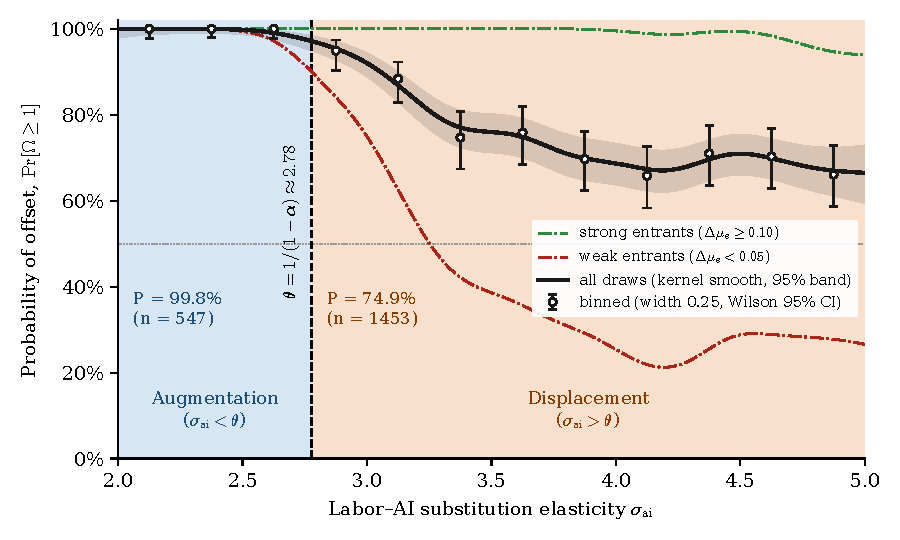
\includegraphics[width=\linewidth]{sigma_threshold}
  \caption{Probability of offset as a function of the labor--AI substitution elasticity.
    Each Monte Carlo draw counts as an offset when the net employment effect is positive. When large-firm (500+) employment falls, this is the same event as $\Omega \ge 1$: gains at firms below 500 employees cover the loss at large firms.
    Points are 0.25-wide bins of $\sigma_{\text{ai}}$ with Wilson 95\% intervals; the solid line is a Gaussian-kernel smooth (bandwidth 0.15) with a 95\% band; dash-dotted lines repeat the smooth for draws with weak ($\Delta\mu_e < 0.05$) and strong ($\Delta\mu_e \ge 0.10$) AI-native entrants.
    The dashed vertical line is the single-firm displacement threshold $\theta = 1/(1-\alpha) \approx 2.78$ (\cref{eq:threshold}).
    In the augmentation region ($\sigma_{\text{ai}} < \theta$) the scale effect dominates, AI raises labor demand at adopting firms, and offset is near-certain (99.8\%, $n = 547$).
    In the displacement region ($\sigma_{\text{ai}} > \theta$) adopters shed workers and offset falls to 74.9\% ($n = 1{,}453$). It levels off near 66--70\% instead of collapsing, because higher $\sigma_{\text{ai}}$ also shrinks AI's cost advantage and so its adoption.
    Above $\theta$, entrant quality decides the outcome: offset stays near 100\% with strong entrants and drops to 20--30\% with weak ones.
    $N = 2{,}000$ draws; data: \texttt{data/monte\_carlo\_raw.csv}; figure: \texttt{scripts/plot\_sigma\_threshold.py}.}
  \label{fig:sigma-threshold}
\end{figure}

The interaction between $\sigma_{\text{ai}}$ and the entrant productivity shift is decisive (\cref{fig:offset-distribution}).
When $\sigma_{\text{ai}} > 3.5$ and the entrant productivity shift is weak ($< 0.05$), P(offset) collapses to 27.8\% ($n = 316$).
When the entrant shift is strong ($\geq 0.10$), P(offset) is 99.3\% pooled across $\sigma_{\text{ai}}$ ($n = 689$), and at least 97\% in every $\sigma_{\text{ai}}$ bin.

\begin{figure}[t]
  \centering
  \fbox{\parbox[c][0.25\textheight][c]{0.8\linewidth}{\centering P(offset) by $\sigma_{\text{ai}}$ bin and entrant productivity shift tercile. At low $\sigma_{\text{ai}}$, offset is universal; at high $\sigma_{\text{ai}}$, entrant quality determines outcome.}}
  \caption{Probability of offset across the parameter space}
  \label{fig:offset-distribution}
\end{figure}

\paragraph{Implications for monitoring.}
These results suggest that policymakers and researchers should monitor two quantities as AI diffuses:
\begin{enumerate}
  \item \textbf{Employment at AI-adopting establishments}---direct evidence on whether $\sigma_{\text{ai}}$ is above or below the threshold. Early survey evidence (BTOS October 2026: only 2\% of adopters reduced employment) suggests $\sigma_{\text{ai}}$ is currently below the threshold.
  \item \textbf{Productivity and employment at AI-native entrants}---whether the firms being created with AI are more productive than counterfactual entrants, and how many workers they employ per dollar of output.
\end{enumerate}

\paragraph{Robustness.}
Fixed-parameter replications (60 runs at $\sigma_{\text{ai}} = 3.5$, a 20\% entry-cost cut, $\Delta\mu_e = 0.05$, and $F_{\text{ai}} = 5$) give a net employment effect with mean $+3.3\%$ and standard deviation $4.2\%$, indicating that simulation noise accounts for roughly 6\% of the total variance in the Monte Carlo.
Noise matters more where the effect is small: for $\sigma_{\text{ai}} \ge 3.25$ it accounts for about a quarter of the variance, so P(offset) in that region mixes parameter uncertainty with finite-economy luck.
The smoothed response surface (quartic polynomial, $R^2 = 0.93$) gives P(offset) = 83.2\%, confirming that the headline is not driven by noise.

\section{Empirical Signatures}\label{sec:signatures}

% Role: testable predictions that separate offsetting entry from pure displacement, each mapped to data.

The model implies a set of predictions that distinguish two hypotheses.
Under \emph{pure displacement}, AI lowers employment at large incumbents with no offsetting response at the entry margin.
Under \emph{offsetting entry}, the same shock also lowers the cost of starting and running a firm, so entry and employment in the band $\Bc$ rise in AI-exposed industries.
Each prediction below is stated relative to less-exposed industries in the same country and year.

\begin{prediction}[Incumbent headcount]\label{pred:incumbent}
Employment at firms that were large before the shock falls in AI-exposed industries.
This prediction holds under both hypotheses and serves as a check that the exposure measure captures the displacement channel.
\end{prediction}

\begin{prediction}[Entry]\label{pred:entry}
Firm entry rates rise in AI-exposed industries relative to their pre-shock trend.
Under pure displacement, entry does not respond, or falls if displaced workers face weaker demand for their skills.
\end{prediction}

\begin{prediction}[Entrant size]\label{pred:entrant-size}
Average employment at entry falls, because the AI task share $\phi$ also applies to entrants, while the number of entrants rises.
\end{prediction}

\begin{prediction}[Employment in the band]\label{pred:band}
Employment at firms in the band $\Bc$, classified by pre-shock size and including entrants, rises in AI-exposed industries.
The offset ratio $\Omega$ in \cref{eq:offset-ratio} is the ratio of this response to the response in \cref{pred:incumbent}.
\end{prediction}

\begin{prediction}[Capital required at entry]\label{pred:capital}
The amount of external capital raised before a firm's first product falls in AI-exposed sectors, by analogy with the cloud era \citep{ewens2018cost}.
\end{prediction}

\begin{prediction}[Transatlantic differences]\label{pred:us-europe}
The employment response in the band $\Bc$ is larger in the United States than in Europe, and the gap appears mainly in the post-entry growth of AI-exposed entrants rather than in entry rates.
Europe's employer start-up rate is about half the US rate, its employment protection is about three times as strict, and its private AI investment is roughly a tenth of the US level; formal start-up registration costs, by contrast, are not systematically higher \citep{eurostat2026bdsize,oecd2020epl,oecd2024pmr,hai2026aiindex}.
The AI Act raises fixed compliance costs for entrants in high-risk uses \citep{euaiact2024}.
In a stylized European parameterization of the Monte Carlo (\cref{sec:disc-europe}), the probability of offset falls from 82\% to 70\%, mostly through thinner scale-up finance for AI-native entrants rather than through entry costs.
The transatlantic difference remains smaller than the uncertainty in $\sigma_{\text{ai}}$ (\cref{tab:sensitivity}).
\end{prediction}

\Cref{tab:signatures} maps each prediction to candidate US and European data sources.

\begin{table}[t]
  \centering
  \caption{Empirical signatures and candidate data sources}
  \label{tab:signatures}
  \begin{tabular}{lll}
    \toprule
    Prediction & United States & Europe \\
    \midrule
    \ref{pred:incumbent}.\ Incumbent headcount & BDS; BTOS (Oct 2026: 2\% cut) & Community Survey on ICT \\
    \ref{pred:entry}.\ Entry & BFS (2025: +62\% vs.\ 2019) & Eurostat business demography \\
    \ref{pred:entrant-size}.\ Entrant size & BDS; BFS (WBA share 2026: 6.8\%) & OECD DynEmp \\
    \ref{pred:band}.\ Band employment & Business Dynamics Statistics & Eurostat SBS \\
    \ref{pred:capital}.\ Capital at entry & PitchBook, Crunchbase & Dealroom \\
    \ref{pred:us-europe}.\ Transatlantic gap & \multicolumn{2}{c}{Harmonized via OECD DynEmp} \\
    \bottomrule
  \end{tabular}
  \par\smallskip
  \parbox{\linewidth}{\footnotesize BFS figures from \citet{bfs2026}: business applications in 2025 relative to 2019, and applications with planned wages (WBA) as a share of all applications, January--September 2026. BTOS figure from \citet{btos2026oct}.}
\end{table}

\paragraph{AI exposure measure.}
We measure AI exposure at the industry level using task-based scores from \citet{eloundou2024gpts} and \citet{felten2021occupational}, mapped to NAICS (US) and NACE (Europe) via crosswalks.
\placeholder{Report the range of industry exposure scores once the crosswalk is computed. The simulation uses relative exposures of 0.5 (goods production), 0.8 (trade and transport), 1.2 (professional services), and 1.5 (information and finance), an ordering consistent with AI use rates by sector in BTOS and Eurostat.}
To ensure the measure is predetermined, we use scores published before 2024 and verify that pre-shock trends in outcomes do not correlate with exposure; \cref{tab:bfs-tests} reports this check for business applications.

\paragraph{Pre-trends and placebos in business applications.}
A first test of \cref{pred:entry} uses the Census Business Formation Statistics \citep{bfs2026}: seasonally adjusted monthly applications for 19 NAICS sectors through September 2026.
We estimate a two-way fixed-effects event study of log applications, with Information (NAICS 51) and Professional services (54) as the exposed group, the 15 sectors outside the exposed and placebo groups as controls, and 2022 as the base year.
Before the shock the exposed sectors track the controls closely.
Their differential trend over 2010--2022 is $-0.3\%$ per year (s.e.\ $1.0\%$), every 2015--2021 event coefficient lies between $-0.01$ and $0.09$ log points, and a fictitious shock dated 2016, estimated on pre-COVID data, yields $-0.001$ (s.e.\ $0.053$).
Hence the post-shock gap is not the continuation of a pre-existing divergence.
The response is also not immediate.
The gap is $-0.03$ in 2023 and $0.00$ in 2024; it opens in March 2025 and widens almost monotonically to $0.34$ log points (about $+41\%$) by September 2026 (\cref{fig:bfs-gap}).
The 2026 coefficient of $0.29$ (s.e.\ $0.06$) ranks 10th of the 171 sector pairs that could have been labelled ``exposed'' (one-sided permutation $p = 0.06$), whereas the same statistic for 2015--2021 never ranks above 40th.
Construction, a low-exposure sector, is a clean placebo: its gap stays within $\pm 0.01$ of zero in every year from 2023 to 2026.
Retail is not a clean placebo, because it carries a $+3.8\%$ annual pre-trend from the e-commerce wave and erratic single-month spikes after 2024; we report it in \cref{tab:bfs-tests} for transparency.
Two qualifications follow from the same data.
First, the divergence is confined to applications with a low propensity to hire: for high-propensity applications the 2026 coefficient is $0.12$ (s.e.\ $0.12$) and ranks 48th, and Information alone is negative.
This agrees with \cref{pred:entrant-size} but does not yet show employer entry.
Second, because 2023--2024 show no effect, a pooled 2023--2026 difference-in-differences is small and insignificant ($0.06$, permutation $p = 0.32$); dating the effective shock to 2025, when capable coding and agent tools diffused, fits the data, but that date was chosen after the data were observed.
With two exposed sectors, conventional clustered errors over-reject \citep{conley2011inference}, so we treat the permutation ranks as the primary inference.
Data, code and full tables are in \texttt{data/bfs\_causal\_analysis.md} and \texttt{scripts/bfs\_causal\_analysis.py}.

\begin{figure}[t]
  \centering
  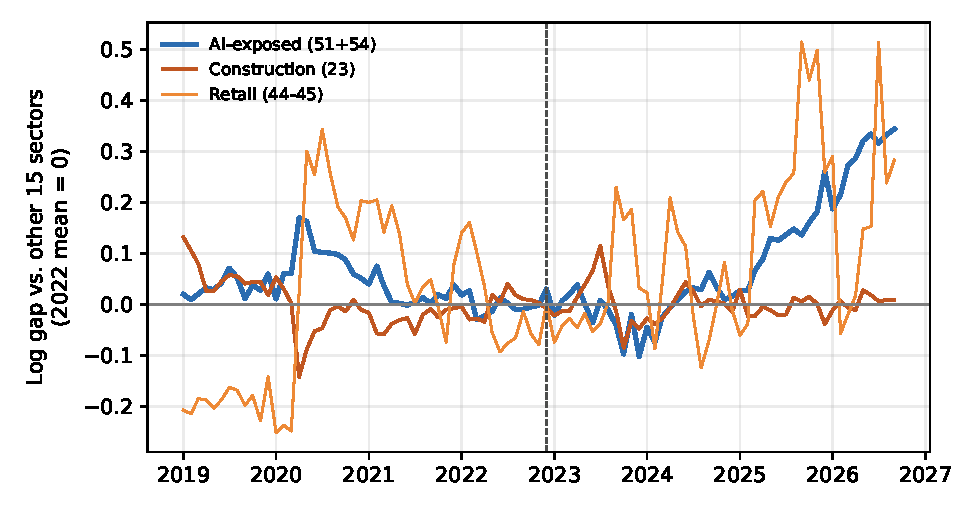
\includegraphics[width=0.85\linewidth]{bfs_monthly_gap}
  \caption{Business applications in AI-exposed sectors relative to other sectors.
    Log gap between seasonally adjusted monthly applications in each group and the mean of the 15 other NAICS sectors, normalized to the 2022 mean.
    AI-exposed is the mean of Information (51) and Professional services (54).
    Dashed line: December 2022.
    \footnotesize\textit{Source: Census BFS, January 2019--September 2026; our calculations.}}
  \label{fig:bfs-gap}
\end{figure}

\begin{table}[t]
  \centering
  \caption{Pre-trend, placebo and permutation tests: log business applications}
  \label{tab:bfs-tests}
  \begin{tabular}{lcccc}
    \toprule
     & Pre-trend & Fake shock & Event coef. & Rank of 2026 \\
     & 2010--22 (\%/yr) & 2016 & 2026 & among 171 pairs \\
    \midrule
    \multicolumn{5}{l}{\textit{All applications}} \\
    Information + Professional (51, 54) & $-0.26$ \, (1.0) & $-0.001$ \, (0.053) & $0.292$ \, (0.059) & 10 \\
    Placebo: Construction (23)          & $2.26$           & $0.189$              & $0.005$              & -- \\
    Placebo: Retail (44--45)            & $3.81$           & $0.093$              & $0.187$              & -- \\
    \multicolumn{5}{l}{\textit{High-propensity applications}} \\
    Information + Professional (51, 54) & $-0.21$ \, (1.0) & $0.020$ \, (0.058)  & $0.116$ \, (0.124)  & 48 \\
    \bottomrule
  \end{tabular}
  \par\smallskip
  \parbox{\linewidth}{\footnotesize Two-way (sector, year) fixed effects; controls are the 15 other NAICS sectors; base year 2022; 2026 is January--September.
    Standard errors clustered by sector in parentheses (reported for the two-sector group only).
    Fake shock: 2016--2019 vs.\ 2010--2015.
    Rank: position of the group's 2026 gap (relative to 2022, against the other 17 sectors) among all $\binom{19}{2} = 171$ sector pairs, 1 = largest.
    \textit{Source: Census BFS; our calculations.}}
\end{table}

\section{Discussion}\label{sec:discussion}

% Role: where the cloud analogy breaks, limitations of the design, and policy implications.

\subsection{The two-layer structure of AI employment}\label{sec:disc-layers}

The AI economy has a two-layer structure that inverts the cloud-era pattern and complicates the offset hypothesis.
We distinguish \emph{AI infrastructure providers}---frontier labs (OpenAI, Anthropic), hyperscalers (Microsoft, Google, Amazon), and neoclouds (CoreWeave)---from \emph{AI application companies} that consume AI APIs without training their own models (Cursor, Lovable, Vercel).
This distinction matters because the offset mechanism, if it operates, must work through the application layer; the infrastructure layer is a special case that does not generalize.

\paragraph{Labs as the ``hyperscalers of AI.''}
Frontier AI labs are analogous not to Databricks (a cloud \emph{user}) but to AWS itself---infrastructure providers on which other companies build.
Anthropic's October 2026 S-1 reports compute and infrastructure costs equal to 48\% of revenue in the second quarter of 2026 \citep{anthropic2026s1}, with spending flowing to chip manufacturers (Nvidia), hyperscalers (AWS, Google Cloud), and data-center construction.
The employment these firms create lands largely at old, large firms---Nvidia, Microsoft (about 223,000 employees as of June 2026; \citealp{techcrunch2026msftbuyout}), and Alphabet (roughly 190,000)---not at the labs themselves.
Labs are capital-intensive, not labor-intensive, and their growth does not test the offset hypothesis for the broader economy.

\paragraph{Hyperscaler capex-for-headcount substitution.}
Microsoft offers the clearest case of a hyperscaler cutting headcount while expanding capital spending.
On October 26, 2026 it extended a voluntary exit offer to about 60,000 employees---roughly a quarter of its workforce---at vice-president level and below in the United States, Canada, India, and the United Kingdom, with some data-center, sales, and marketing staff reportedly excluded \citep{techcrunch2026msftbuyout}.
This is an eligibility figure, not an exit count; uptake had not been reported at the time of writing.
The offer follows roughly 9,000 layoffs (just under 4\% of the workforce) beginning in July 2025 \citep{verdict2025msftlayoffs}, and a 2\% year-over-year decline in total headcount in fiscal 2026 \citep{msft2026fy26q4}.
Over the same period capital expenditure rose steeply: from a planned \$80 billion for AI-enabled data centers in fiscal 2025 \citep{smith2025golden} to \$41 billion in the June 2026 quarter alone, with calendar-2026 capex guided to approximately \$175 billion \citep{msft2026fy26q4}.
The pattern is consistent with Microsoft trading headcount for data-center capacity---the substitution dynamic our model describes at incumbents, here occurring at the infrastructure layer itself---although Microsoft frames the program as retooling its workforce for AI, and these aggregate figures cannot establish that capex is causing the exits.
More broadly, Bridgewater reportedly estimates that Alphabet, Amazon, Meta, and Microsoft will spend about \$650 billion on AI infrastructure in 2026, up from about \$410 billion in 2025 \citep{hedgeco2026bridgewater}; we were unable to obtain Bridgewater's original publication.

\paragraph{Neocloud capital constraints.}
The ``neocloud'' model (purpose-built AI infrastructure competing with hyperscalers) is not a broad employment channel.
% [claim] CoreWeave figures (headcount, revenue, debt, customer share) currently rest on Wikipedia; cite CoreWeave's 10-K/10-Q directly.
CoreWeave, the leading neocloud, had 2,189 employees servicing \$5.13 billion in revenue (2025)---\$2.3 million per employee.
More critically, CoreWeave carries \$35.1 billion in debt (June 2026) collateralized against contracts with hyperscalers (Microsoft represents 67\% of revenue).
Without similar anchor contracts the barrier to entry for new neoclouds is high, so the slipstream behind hyperscaler infrastructure spending is narrow.

\subsection{AI application companies: the real test}\label{sec:disc-applications}

If the offset hypothesis has empirical content, it must operate through \emph{AI application companies}---firms that use AI APIs to build products, analogous to how Databricks used AWS.
The evidence from this layer does not support offset in employment terms.

\paragraph{Employment-light application firms.}
% [claim] Cursor and Lovable figures rest on press reports aggregated by Wikipedia and Dealroom; cite the underlying Bloomberg/TechCrunch/Forbes articles.
Cursor, which uses Claude and GPT-4 APIs to build an AI coding assistant, reached \$3 billion in annualized recurring revenue (May 2026) with approximately 300 employees---\$10 million in revenue per employee.
Lovable, a Swedish ``vibe coding'' platform, reached \$200 million ARR (November 2025) with about 120 employees (\$1.7 million per employee).
The cloud-era SaaS comparators in \cref{tab:ai-vs-cloud} operated at \$0.17--0.32 million per employee, and cloud-era SaaS firms generally at roughly \$0.25--0.45 million; Cursor's ratio is more than twenty times higher, and Lovable's five to ten times higher.
The AI application layer is growing rapidly, but each firm absorbs little labor.

\paragraph{Exit path disruption.}
The graduation pathway that fed young-firm employment into the large-firm stock is being short-circuited by mega-acquisitions.
% [claim] Acquisition facts (SpaceX--Cursor, SpaceX--xAI, Microsoft--Inflection, Google--Character.ai) need press or filing citations.
SpaceX acquired Cursor for \$60 billion in August 2026; SpaceX also absorbed xAI (\$250 billion) in February 2026.
Microsoft absorbed Inflection's staff in March 2024; Google licensed Character.ai and rehired its founders.
In BDS terms, when SpaceX (founded 2002, age 24) acquires Cursor (founded 2022, age 4), Cursor's employees become ``old large firm'' employment.
The young high-growth firms that \citet{haltiwanger2013who} credit with job creation are not surviving long enough to graduate as independent employers.

\subsection{More firms, not more employers}\label{sec:disc-augment}

The distinction between \emph{offset} (new firms creating jobs that replace those lost at incumbents) and \emph{employment-light formation} (new firms that produce with few or no employees) is empirically critical.

Business Formation Statistics show record business applications, up 15.3\% in January--September 2026 relative to the same months of 2025, with Information sector applications up 39.8\% \citep{bfs2026}.
Yet applications with planned wages---a proxy for intent to become an employer---fell 15.3\% over the same period.
In Information, planned-wage applications fell from 12.3\% of total applications in 2019 to 4.8\% in 2026.
Formation is responding at the firm-count margin, but not yet at the employer margin; this matches the event-study evidence in \cref{sec:signatures}, where the divergence of AI-exposed sectors is confined to low-propensity applications.
Two caveats apply.
The decline in planned-wage applications appears in every sector, so it is not specific to AI; and it continues a cloud-era trend, when such applications fell 48\% between 2006 and 2019 (\cref{sec:cloud-findings}).
The pattern is nonetheless the one the model predicts when AI also applies to entrants (\cref{pred:entrant-size}): more firms, but fewer jobs per firm.

\subsection{Implications for the original offset hypothesis}\label{sec:disc-offset-revised}

\Cref{tab:ai-vs-cloud} summarizes the employment-intensity comparison.
The evidence suggests that even if AI-native firm formation flourishes, the employment consequences differ fundamentally from the cloud era.
Cloud computing reduced the cost of starting firms that then \emph{hired workers as they scaled}.
AI reduces the \emph{need for workers} at firms that scale.
The offset ratio $\Omega$ may approach unity in firm counts while remaining well below unity in employment.

\begin{table}[t]
  \centering
  \caption{Valuation and revenue per employee: AI vs.\ cloud-era firms}
  \label{tab:ai-vs-cloud}
  \begin{tabular}{llrrrr}
    \toprule
    Company & Layer / Era & Valuation & Revenue & Employees & Rev./Emp. \\
    \midrule
    \multicolumn{6}{l}{\textit{AI Infrastructure (labs, neoclouds)}} \\
    Anthropic (S-1, Oct 2026) & Lab & $\sim$\$1T & \$35B TTM & 5,300 & \$6.6M \\
    OpenAI (2026) & Lab & \$840B & \$12B est. & 4,500 & \$2.7M \\
    CoreWeave (2025) & Neocloud & \$27B & \$5.1B & 2,189 & \$2.3M \\
    \midrule
    \multicolumn{6}{l}{\textit{AI Applications (API consumers)}} \\
    Cursor (May 2026) & Application & \$60B & \$3B ARR & 300 & \$10.0M \\
    Lovable (2025--26) & Application & \$13.3B & \$200M ARR & 120 & \$1.7M \\
    Vercel (Sep 2025) & Application & \$9.3B & \$300M est. & 550 & \$0.5M \\
    \midrule
    \multicolumn{6}{l}{\textit{Cloud-era SaaS (baseline)}} \\
    Databricks (2021) & Cloud SaaS & \$38B & \$1.6B & 5,000 & \$0.32M \\
    Snowflake (2020 IPO) & Cloud SaaS & \$70B & \$0.6B & 3,500 & \$0.17M \\
    \bottomrule
  \end{tabular}
  \smallskip
  \footnotesize\textit{Sources: Anthropic S-1 \citep{anthropic2026s1}; Cursor/Lovable/CoreWeave from Wikipedia citing Bloomberg, TechCrunch. Lovable valuation as of August 2026, revenue and headcount as of late 2025. Cloud-era figures from company filings at comparable stages.}
  % [claim] Replace Wikipedia with primary sources and verify the cloud-era rows (Databricks 2021, Snowflake 2020) against filings.
\end{table}

\subsection{How AI differs from cloud computing}\label{sec:disc-differences}

Beyond the two-layer structure, AI differs from cloud computing in ways that affect the offset ratio even within the application layer.

\paragraph{Direct evidence from the S-1: AI as augmentation inside Anthropic.}
Anthropic's October 2026 S-1 \citep{anthropic2026s1} provides evidence, disclosed under securities law, on how a frontier AI lab views its own technology's effect on labor.
The filing reveals that ``over 90\% of the contributions to [Anthropic's] codebase in September 2026 were written by Claude,'' and that ``the average daily volume of code contributed per engineer'' rose 45$\times$ from 2024 to 2026.
Yet the company grew from about 940 employees (December 2024) to about 5,300 (September 2026)---\textit{employment rose alongside AI-driven productivity gains}, the pattern the model associates with $\sigma_{\text{ai}} < \theta$ rather than displacement, although a single fast-growing firm cannot identify $\sigma_{\text{ai}}$.
The filing explicitly frames Claude as enabling ``a comparatively small team to take on work that would traditionally require a far larger one,'' describing this as ``multiplying the impact of each person'' rather than replacing workers.

Anthropic's risk factors acknowledge the displacement concern as a regulatory and reputational risk: the company warns that governments ``may intervene to slow the rate of adoption of AI'' if ``the rate of job displacement rapidly increases,'' and that it ``may from time to time voluntarily elect to take actions intended to ameliorate the impact of such displacement''---actions that ``would represent additional costs and expenditures for which [it] may not receive a corresponding commercial benefit.''
To our knowledge, this is the first disclosure in a securities filing by a frontier lab that it views labor-displacement backlash as a material business risk that may require mitigation.

\paragraph{Breadth of exposure.}
% [claim] breadth relative to cloud needs a direct comparison, not only AI exposure scores.
The effects of cloud computing were concentrated in sectors that relied heavily on computing, whereas measures of exposure to large language models span a wide range of occupations \citep{eloundou2024gpts}.
A broader shock raises both displacement and the scope for entry, so its net effect on $\Omega$ is ambiguous.

\paragraph{Complementary investments and timing.}
General-purpose technologies require complementary intangible investments before they raise measured productivity \citep{brynjolfsson2021productivity}.
If incumbents capture these gains before entrants can, the displacement channel leads the entry channel, which reinforces the timing problem described in \cref{sec:intro}.

\paragraph{Market structure of the input.}
The AI input market is highly concentrated: as of 2026, foundation model development is dominated by a handful of labs (OpenAI, Anthropic, Google DeepMind, Meta AI), and compute capacity is controlled by a small number of cloud providers and chip manufacturers.
This concentration may allow non-competitive pricing of AI services, raising the price $r$ and hence lowering $w/r$ in \cref{eq:displacement-condition} below what a commodity market would deliver.
If AI services are priced above marginal cost, the productivity effect of a given task share shrinks and fewer firms clear the adoption cutoff in \cref{eq:adoption-cutoff}; in the CES specification the threshold $\theta$ itself is unaffected, so supra-competitive pricing scales down AI's employment effects rather than changing their sign.
However, concentration also creates hold-up risk for AI-dependent entrants, potentially raising effective entry barriers despite lower technical costs of starting a firm.

\subsection{Europe: a transatlantic comparison}\label{sec:disc-europe}

\Cref{pred:us-europe} predicts a smaller entry response in Europe.
This subsection checks the premises of that prediction against data, sets out what the AI Act changes at the entry margin, and asks whether the offset mechanism is more or less likely to operate in Europe.
\Cref{tab:us-europe} summarizes the comparison; underlying computations and sources are in \texttt{data/europe\_evidence.md}.

\begin{table}[t]
  \centering
  \caption{United States vs.\ Europe: entry, finance, regulation, and labor-market rigidity}
  \label{tab:us-europe}
  \small
  \begin{tabular}{p{4.6cm}p{4.3cm}p{5.4cm}}
    \toprule
    Dimension & United States & European Union \\
    \midrule
    \multicolumn{3}{l}{\textit{Business formation}} \\
    Employer start-up rate & 9.1\% (2023) & 4.8\% (2024); 5.2\% (2021) \\
    \quad in ICT / Information & 12.0\% (NAICS 51, 2022) & 6.4\% (NACE J, 2024); 7.7\% (2022) \\
    Births with no employees & n/a (nonemployer series) & 84\% of all births (2024) \\
    \midrule
    \multicolumn{3}{l}{\textit{AI finance and adoption}} \\
    Private AI investment, 2025 & \$285.9B & \$20.9B (ratio $\approx$ 14); 9--12$\times$ in Crunchbase/Dealroom \\
    AI use, large vs.\ small firms & 1.7$\times$ (250+ vs.\ 1--4) & 3.2$\times$ (250+ vs.\ 10--49, 2025) \\
    \midrule
    \multicolumn{3}{l}{\textit{Entry costs and regulation}} \\
    Admin.\ burden on start-ups (PMR, 0--6) & 2.03 & 1.11 (SE) -- 2.74 (DE); FR 1.60, IT 1.80 \\
    AI-specific horizontal regulation & None at federal level & AI Act; high-risk duties from Dec 2027 \\
    \midrule
    \multicolumn{3}{l}{\textit{Labor-market rigidity}} \\
    EPL, regular contracts (0--6) & 0.77 & 1.94 (DK) -- 2.88 (NL); DE 2.33, FR 2.68, IT 2.86 \\
    \bottomrule
  \end{tabular}
  \smallskip

  \footnotesize\raggedright\textit{Sources:} US start-up rates from the Business Dynamics Statistics \citep{bds2021}; EU employer start-up rate = births with $\geq 1$ employee $\div$ active enterprises with $\geq 1$ employee, business economy excl.\ holding companies \citep{eurostat2026bdsize}.
  AI investment from \citet{hai2026aiindex}, with \citet{dealroom2026ai} as a cross-check; adoption ratios from BTOS \citep{btos2026oct} and \citet{eurostat2026isoc} (EU survey excludes firms with fewer than 10 persons employed).
  PMR indicator ``administrative requirements for limited liability companies and personally owned enterprises'' \citep{oecd2024pmr}; EPL Version 4, individual and collective dismissals, 2019 \citep{oecd2020epl}.
  Levels are not strictly comparable across the Atlantic (enterprise vs.\ firm units; persons employed vs.\ employees).
\end{table}

\paragraph{Business formation.}
Europe forms employers at roughly half the US rate.
In 2024, 4.8\% of EU-27 enterprises with at least one employee were newly born, against a BDS start-up rate of 9.1\% in 2023 \citep{eurostat2026bdsize,bds2021}.
The EU's headline birth rate (10.4\%) looks higher only because 84\% of European births have no employees.
The early generative-AI years also differ in direction.
US business applications surged, led by the Information sector (\cref{sec:disc-augment}).
In the EU, employer births in information and communication \emph{fell} from 7.7\% (2022) to 6.4\% (2024), and in computer programming (J62) from 8.9\% to 7.0\%, while the zero-employee share of births edged up.
Europe therefore shows the employment-light composition seen in the United States, without the US surge in formation.
Harmonized DynEmp evidence adds that young firms are the main source of net job creation in every country covered, but that the post-entry growth of surviving start-ups varies widely across countries and is tied to national policy \citep{criscuolo2014dynamics,calvino2016no}; business dynamism has also declined across OECD economies, mainly within sectors \citep{calvino2020declining}.

\paragraph{AI start-up funding.}
In 2025, private AI investment was \$285.9 billion in the United States against \$20.9 billion in Europe \citep{hai2026aiindex}, a ratio of about 14.
Other databases put the ratio at 9 to 12, and the gap is concentrated in growth and late-stage rounds, where more than half of European AI capital comes from non-European, mostly US, investors \citep{dealroom2026ai}.
Europe has produced AI-native application firms (Lovable in \cref{tab:ai-vs-cloud}), but the capital that lets an entrant scale to the band $\Bc$ is far thinner.
In the model, this maps most naturally to a smaller productivity advantage for AI-native entrants, the parameter that decides offset once $\sigma_{\text{ai}}$ exceeds the displacement threshold (\cref{sec:simulation}).

\paragraph{Entry costs: the premise needs refining.}
\Cref{pred:us-europe} assumed that general entry costs are higher in Europe.
The OECD's product-market regulation indicators do not support this.
On the administrative requirements for setting up a limited liability company or a sole proprietorship, the United States scores 2.03 on a 0--6 scale, above France (1.60), Italy (1.80), Spain (1.39), and Sweden (1.11), and below only Germany (2.74) and the Netherlands (2.21) \citep{oecd2024pmr}.
The US economy-wide PMR score (1.58) is higher than that of every large EU economy.
The transatlantic gap in employer formation is therefore not explained by registration costs.
It lines up with three other differences: employment protection, scale-up finance, and, prospectively, AI-specific regulation.

\paragraph{The AI Act and the entry margin.}
The AI Act \citep{euaiact2024} adds a cost that has no US federal counterpart, and its incidence differs by firm size.
Its core obligations for high-risk systems (risk management, data governance, technical documentation, human oversight, a quality-management system, and conformity assessment) are largely fixed costs: they scale with the number of systems a firm places on the market, not with its headcount.
Estimates prepared for the Commission put aggregate compliance costs at 4--5\% of investment in high-risk AI, plus 2--5\% for verification \citep{ec2021aiactia}; independent estimates put the set-up cost of a new quality-management system at roughly EUR~193,000--330,000, with about EUR~71,000 a year to maintain it \citep{laurer2021clarifying}.
An incumbent with established compliance functions (ISO management systems, GDPR, sectoral regulation) absorbs much of this within existing processes; for a five-person entrant the same outlay can be comparable to its seed round.
In the notation of \cref{sec:ai-entry}, the Act raises $\kappa_e$ for entrants in high-risk uses and raises the fixed cost of adoption, partly offsetting the reduction in entry costs that AI otherwise delivers.

Three features limit this effect.
First, the Act is proportionate by design: for SMEs and start-ups each fine is capped at the \emph{lower} of the percentage-of-turnover and fixed-amount ceilings (Art.~99(6)), conformity-assessment fees are reduced in proportion to size, and SMEs get priority access to regulatory sandboxes (Art.~62) and simplified technical documentation (Art.~11).
The Digital Omnibus on AI \citep{euaiomnibus2026} extended these privileges to small mid-caps (fewer than 750 employees), which covers much of the band $\Bc$ in European size terms.
Second, incidence is narrow: most AI-application start-ups (coding tools, marketing, productivity software) fall outside the high-risk categories in Annex~III and face only the transparency duties of Art.~50.
The exposure is concentrated in employment, credit, education, and essential-services applications, where an entrant's product \emph{is} the high-risk system.
Third, timing: the Omnibus deferred stand-alone high-risk obligations from August 2026 to December 2027, and obligations for AI embedded in regulated products to August 2028.
The Act's main cost so far is uncertainty rather than compliance outlays: among EU enterprises that considered using AI, 52.5\% cited unclear legal consequences as a barrier \citep{eurostat2026isoc}.

\paragraph{Labor-market rigidity.}
The largest structural difference is employment protection.
On the OECD's index for individual and collective dismissals of regular workers, the United States scores 0.77, against 2.33 in Germany, 2.68 in France, 2.86 in Italy, and an OECD average of 2.20 \citep{oecd2020epl}.
Firing costs act on both sides of the offset ratio $\Omega$.
In the denominator, they slow the rate at which AI-adopting incumbents can shed labor; adjustment then runs through attrition and hiring freezes rather than layoffs, and the measured loss at incumbents is smaller and later \citep{hopenhayn1993job}.
In the numerator, they also slow entrants' scale-up: stricter employment protection is associated with a less dynamic firm-growth distribution, with fewer fast-growing young firms, in labor- and R\&D-intensive sectors \citep{bravobiosca2016drives}.
Because AI-native entrants are already employment-light, the second effect weighs on precisely the hiring that offset requires.

\paragraph{Is offset more or less likely in Europe?}
To gauge the combined effect, we rerun the Monte Carlo of \cref{sec:simulation} under a stylized European parameterization, holding the technology draws ($\sigma_{\text{ai}}$), the uniform quantiles of every other prior, and the simulation seeds fixed across scenarios, so that differences reflect institutions only.
Each European channel is switched on in turn:
(i) a potential-entrant pool scaled by 0.53, the ratio of the EU employer birth rate to the US start-up rate;
(ii) AI Act compliance, which caps the AI-induced entry-cost reduction at 20\% (against 30\%) and raises the adoption fixed cost from $U(2,10)$ to $U(3,12)$;
(iii) thinner growth finance, which caps the AI-native entrant productivity shift at 0.10 (against 0.15).
\Cref{tab:eu-mc} reports the results; the US scenario reproduces the headline probability of \cref{sec:simulation}.

\begin{table}[t]
  \centering
  \caption{Offset under US and stylized European parameterizations}
  \label{tab:eu-mc}
  \small
  \begin{tabular}{lcccc}
    \toprule
    Scenario & $P(\text{offset})$ & $P(\text{offset} \mid \sigma_{\text{ai}} > 2.78)$ & Median net effect & Mean diff.\ vs.\ US (pp) \\
    \midrule
    United States & 81.7\% & 75.3\% & $+9.7\%$ & --- \\
    EU: smaller entry pool & 80.5\% & 74.1\% & $+9.8\%$ & $-0.2$ (0.3) \\
    EU: AI Act costs & 79.3\% & 72.0\% & $+8.4\%$ & $-1.3$ (0.1) \\
    EU: thinner growth finance & 73.1\% & 63.6\% & $+5.2\%$ & $-4.3$ (0.2) \\
    EU: all channels & 69.7\% & 59.3\% & $+4.8\%$ & $-5.5$ (0.3) \\
    \bottomrule
  \end{tabular}
  \smallskip

  \footnotesize\raggedright\textit{Notes:} 1,000 draws per scenario with common random numbers; offset means the net employment effect is positive.
  Standard errors of the paired difference in parentheses.
  Generated by \texttt{scripts/europe\_comparison.py}; full output in \texttt{data/europe\_comparison.md}.
  The model has no firing costs, so the EPL channel is not included.
\end{table}

Three results stand out.
First, offset is less likely in Europe: with all channels on, $P(\text{offset})$ falls from 81.7\% to 69.7\%, and from 75.3\% to 59.3\% in the displacing region $\sigma_{\text{ai}} > 2.78$; offset fails in 15.8\% of draws where it holds under US parameters.
Second, the gap comes mainly from growth finance, not from entry costs.
A smaller founder pool barely moves the proportional employment effect, and AI Act compliance costs lower the net effect by 1.3 percentage points; thinner scale-up finance accounts for most of the 5.5-point gap.
This mirrors the variance decomposition for the United States, in which entrant productivity matters six times as much as the entry-cost cut.
Third, the AI Act's effect is real but second-order at the aggregate level, consistent with its narrow incidence.
Its bite is sector-specific: in the high-risk categories, which overlap the information, finance, and professional-services sectors where displacement is largest, the Act raises entry costs precisely where offset is most needed.

These magnitudes are illustrative.
The mappings from data to parameters are stylized, and the omitted EPL channel cuts both ways: it should damp measured displacement at European incumbents (making $\Omega$ easier to reach in the short run) while also slowing the scale-up of entrants (making it harder in the long run).
The qualitative conclusion is robust to that ambiguity.
Europe's lower AI-driven displacement risk in the near term comes from institutions that slow reallocation, not from a stronger entry response, and the channel the model identifies as decisive, AI-native entrants scaling into employers, is the one where Europe is weakest.
For \cref{pred:us-europe}, the testable implication is that the transatlantic gap should appear in post-entry growth (the employment of surviving AI-exposed entrants at ages 3--5, observable in DynEmp-style data) more than in entry rates.

\subsection{Limitations}\label{sec:disc-limitations}

\begin{itemize}
  \item \textbf{Analogue validity.} The cloud era identifies the response of entry to lower fixed costs; it is informative about AI only insofar as $\kappa_e$ and $\kappa_f$ capture how AI changes those costs.
  \item \textbf{Job counts versus job quality.} The offset ratio counts jobs; it is silent on wages, job security, and the matching of displaced workers to new firms.
  \item \textbf{Firms below five employees.} The band $\Bc$ excludes very small firms and nonemployer businesses, which may absorb part of the entry response; we report $\Delta N^{\Sc}$ separately where data allow.
  \item \textbf{Choice of band.} The bounds of $\Bc$ follow data availability, and the Monte Carlo uses smaller, current-size cutoffs (20 and 500 employees; \cref{sec:sim-design}) because the model economy has few very large firms. \placeholder{Report robustness of the offset statistics to alternative cutoffs and to pre-shock cohort classification.}
  \item \textbf{Partial equilibrium.} The baseline simulations hold wages fixed (perfectly elastic labor supply). A finite labor-supply elasticity would damp both gains and losses. General-equilibrium product-market effects (AI raises output, which raises labor demand) are also omitted.
  \item \textbf{Sector heterogeneity.} The Monte Carlo treats sectoral AI exposure as fixed. In reality, high-exposure sectors (information, finance) may never achieve offset while low-exposure sectors (goods production, trade) always do; aggregate results depend on cross-sector labor reallocation, which the model does not endogenize.
\end{itemize}

\subsection{Policy implications}\label{sec:disc-policy}

If the offset ratio depends on entry costs, policies that affect the cost of starting and scaling a firm---licensing, access to finance, and access to AI services and compute---shape the labor-market consequences of AI alongside policies aimed at displaced workers.
In Europe, the AI Act \citep{euaiact2024} raises fixed compliance costs for entrants in high-risk uses, though its SME and small-mid-cap provisions \citep{euaiomnibus2026} narrow the gap with incumbents. The comparison in \cref{sec:disc-europe} suggests that the larger lever for offset in Europe is scale-up finance for AI-native entrants, not the cost of entry.

Our analysis suggests three policy-relevant findings:

\begin{enumerate}
  \item \textbf{Entry-cost reduction alone is not sufficient.} The Monte Carlo shows that entry-cost reduction explains only 3\% of the variance in aggregate employment outcomes, although it explains a quarter of the variance in small-firm employment. Reducing barriers to starting a business will not produce offset if AI is strongly labor-displacing ($\sigma_{\text{ai}} > 2.78$) and AI-native entrants are not substantially more productive. The cloud-era replication (\cref{sec:cloud-mechanism}) adds that the entry pipeline as a whole---the pool of founders and the cost of becoming an employer---matters more than the cost of computing.
  
  \item \textbf{Monitor $\sigma_{\text{ai}}$ empirically.} The displacement threshold is the most policy-relevant unknown. Early survey evidence \citep{btos2026oct} suggests $\sigma_{\text{ai}}$ is currently below the threshold; if this changes, the offset probability falls sharply.
  
  \item \textbf{Sector-specific policies may be warranted.} High-exposure sectors (information, finance) face structural barriers to offset that low-exposure sectors do not. Retraining and labor-mobility programs may be more important than entry-cost reduction in sectors where offset is unlikely regardless of policy.
\end{enumerate}

\section{Conclusion}\label{sec:conclusion}

% Role: restate the question, the answer, and what to watch for as AI diffuses.

This paper asks whether AI-induced firm formation can offset the employment that large incumbents shed as they adopt AI.
We model the AI shock as a combination of displacement at incumbents and lower fixed costs of entry and operation, discipline the second channel using the cloud-computing era, and quantify the conditions for offset through calibration and Monte Carlo simulation.

\paragraph{Main findings.}
Across 2,000 Monte Carlo draws spanning plausible parameter ranges, the probability that AI raises net employment is 81.7\%.
The result is conditional: offset depends on the labor-AI substitution elasticity $\sigma_{\text{ai}}$, which explains 71\% of the variance in employment outcomes, and much of it reflects the absence of displacement rather than compensation for it.
Entry-cost reduction---the mechanism most analogous to cloud computing---explains only 3\%.

Below the displacement threshold ($\sigma_{\text{ai}} < 2.78$), AI is labor-complementary and offset is nearly universal (99.8\%).
Above the threshold, the offset probability falls to 74.9\% and depends heavily on whether AI-native entrants are more productive than their counterfactual selves.
When $\sigma_{\text{ai}} > 3.5$ and the entrant productivity advantage is weak, the offset probability collapses to 27.8\%.

Early empirical evidence is cautiously optimistic: the Census Bureau's BTOS (October 2026) shows that only 2\% of AI-adopting establishments reduced employment due to AI \citep{btos2026oct}, suggesting $\sigma_{\text{ai}}$ is currently below the threshold.
However, leading AI application firms are markedly employment-light---Cursor generates more than twenty times the revenue per employee of cloud-era SaaS firms---and business applications with planned wages are falling even as total applications reach record highs.

\paragraph{What to watch.}
The single most informative empirical signature is employment change at AI-adopting establishments, which directly reveals whether $\sigma_{\text{ai}}$ is above or below the displacement threshold.
Establishment-level data from the Business Trends and Outlook Survey (United States) and the Community Survey on ICT Usage (Europe) can track this as AI diffuses.
A shift from the current 2\% reporting employment reductions toward higher rates would signal that the labor-complementary regime is ending.

\paragraph{Broader implications.}
The standard approach to measuring AI's labor-market effects focuses on task exposure within a fixed set of firms.
Our analysis suggests this approach understates uncertainty: the net effect of AI on employment depends as much on firm creation as on within-firm automation.
Monitoring and forecasting should therefore track business formation, entrant productivity, and entrant employment alongside task automation rates.
The cloud era---which saw concentration rise despite cheaper computing---is a cautionary precedent: even favorable $\sigma_{\text{ai}}$ does not prevent concentration if structural headwinds suppress entry, and if $\sigma_{\text{ai}}$ turns out to be above the threshold, the same headwinds would turn offset into net job loss.


% ---- References --------------------------------------------------------------
\bibliographystyle{plainnat}
\bibliography{references}

\end{document}
